\chapter{Organisation}
Dette afsnit vil give et indblik i strukturen og opbygningen af "Kvindeafdelingen, Svangre- og ultralydsambulatorium" på Hospitalsenheden Horsens. Afsnittet vil belyse, hvilken betydning implementeringen af en ultralyds robotarm vil have for afdelingen som organisation, samt hvilke ændringer dette vil medføre i arbejdsgangen for personalet. \\
Informationer, som er indhentet fra afdelingen på Hospitalsenheden Horsens, vil blive sammenholdt med videnskabelige artikler, i forsøget på at finde en større sammenhæng i problemstillingen omkring arbejdsgener ved ultralydsscannings arbejdet.

Det er valgt, at benyttes Leavitts organisations model \ref{LeavittModel}. Denne model er en diamantmodel, der arbejder med fire organisatoriske hovedelementer, der relaterer sig til hinanden. Hvert hovedelement vil blive belyst i hvert sit underafsnit. 

\begin{figure}[h!]\centering
	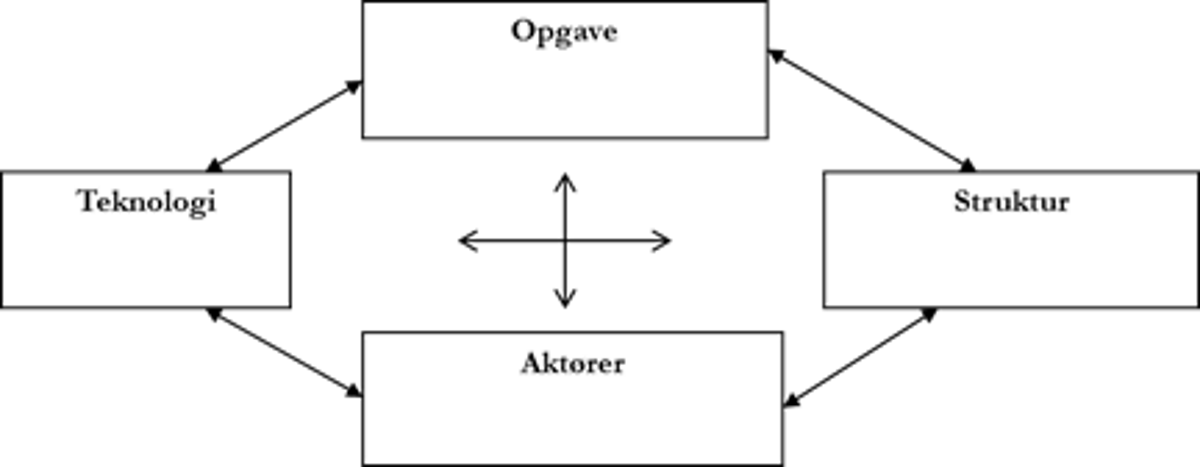
\includegraphics[width = 0.5\textwidth]{Figurer/LeavittModel}
	\caption{Leavitts organisations model, viser hvordan struktur, aktører, opgaver og teknologi indbyrdes relaterer sig til hinanden}
	\label{LeavittModel}
\end{figure}

I denne analyse er der som sagt kun medtaget en enkelt ultralydsafdeling, og derfor er der ikke videre empiri for at kunne drage konklusioner om at billedet vil være det samme på lignende hospitals afdelinger i Danmark. 

\section{Opgaver}


\section{Teknologi}

\section{Struktur}

\section{Aktører}